%%%%%%%%%%%%%%%%%%%%%%%%%%%%%%%%%%%%%%%%%%%%%%%%%%%%%%%%%%%%%%%%%%%%%%%%%
% KHAI BÁO CÁC THÔNG SỐ ĐỀ THI - MÃ ĐỀ 132
%%%%%%%%%%%%%%%%%%%%%%%%%%%%%%%%%%%%%%%%%%%%%%%%%%%%%%%%%%%%%%%%%%%%%%%%%
\def\toanlop{10}
\def\thoigian{45}
\def\namhoc{2024 - 2025}
\begin{dethi}
	{SỞ GD\&ĐT THỪA THIÊN HUẾ}
	{TRƯỜNG THPT CHUYÊN QUỐC HỌC HUẾ}
	{KIỂM TRA GIỮA KÌ I}
	{Thời gian làm bài: 45 phút, không kể thời gian phát đề}
\end{dethi}

\Opensolutionfile{ans}[ans/ansTN-QuocHoc104]

\noindent \textbf{PHẦN I. Câu trắc nghiệm nhiều phương án lựa chọn. Thí sinh trả lời từ câu 1 đến câu 12. Mỗi câu hỏi thí sinh chỉ chọn một phương án}
\vspace{0.2cm}

\begin{ex}%[10V1-104-01]
	Một vật chuyển động thẳng có độ dịch chuyển $d_1$ tại thời điểm $t_1$ và độ dịch chuyển $d_2$ tại thời điểm $t_2$. Vận tốc trung bình của vật trong khoảng thời gian từ $t_1$ đến $t_2$ là
	\choice
	{$v_{tb}=\frac{d_1+d_2}{t_2-t_1}$}
	{$v_{tb}=\frac{1}{2}\left(\frac{d_1}{t_1}+\frac{d_2}{t_2}\right)$}
	{$v_{tb}=\frac{d_1-d_2}{t_1+t_2}$}
	{\True $v_{tb}=\frac{d_2-d_1}{t_2-t_1}$}
	\loigiai{
		Vận tốc trung bình được xác định bằng tỉ số giữa độ dịch chuyển và khoảng thời gian dịch chuyển:
		$$v_{tb} = \frac{\Delta d}{\Delta t} = \frac{d_2 - d_1}{t_2 - t_1}$$
		Chọn D.
	}
\end{ex}

\begin{ex}%[10V1-104-02]
	Khi vật chuyển động thẳng ngược chiều dương thì
	\choice
	{\True Quãng đường có giá trị dương, độ dịch chuyển có giá trị âm}
	{Quãng đường và độ dịch chuyển đều có giá trị âm}
	{Quãng đường và độ dịch chuyển đều có giá trị dương}
	{Quãng đường có giá trị âm, độ dịch chuyển có giá trị dương}
	\loigiai{
		Quãng đường đi được $s$ luôn là một đại lượng vô hướng không âm ($s > 0$). Khi vật chuyển động thẳng ngược chiều dương, tọa độ của vật giảm dần nên độ dịch chuyển $\Delta d = x_2 - x_1 < 0$. Chọn A.
	}
\end{ex}

\begin{ex}%[10V1-104-03]
	Chỉ dùng thước đo chiều dài và đồng hồ bấm giây để đo tốc độ trung bình của một chiếc xe đồ chơi chuyển động thẳng từ điểm A đến điểm B. Nhận định nào sau đây là sai?
	\choice
	{\True Có thể đo trực tiếp được tốc độ trung bình của chuyển động}
	{Dùng thước đo quãng đường $s$ là phép đo trực tiếp}
	{Dùng đồng hồ bấm giây đo thời gian $t$ là phép đo trực tiếp}
	{Dùng công thức $v=\frac{s}{t}$ tính tốc độ trung bình là phép đo gián tiếp}
	\loigiai{
		Tốc độ trung bình được xác định thông qua công thức toán học $v = \frac{s}{t}$ từ các kết quả đo trực tiếp quãng đường $s$ và thời gian $t$, do đó đây là phép đo gián tiếp, không phải phép đo trực tiếp. Nhận định A sai. Chọn A.
	}
\end{ex}

\begin{ex}%[10V1-104-04]
	Cuộc cách mạng công nghiệp lần thứ ba bắt đầu vào những năm 70 của thế kỉ XX là nhờ có những thành tựu nghiên cứu về
	\choice
	{công nghệ vật liệu nano và Vật lí hạt nhân}
	{internet toàn cầu, robot và vật liệu siêu nhỏ}
	{hiện tượng cảm ứng điện từ và dòng điện}
	{\True điện tử, chất bán dẫn và vi mạch}
	\loigiai{
		Cuộc cách mạng công nghiệp lần thứ ba (vào dải những năm 1970) gắn liền với sự ra đời và phát triển vượt bậc của ngành điện tử, chất bán dẫn, vi mạch điện tử và máy tính kĩ thuật số nhằm tự động hóa sản xuất. Chọn D.
	}
\end{ex}

\begin{ex}%[10V1-104-05]
	Sai số tỉ đối của phép đo là
	\choice
	{tỉ số giữa sai số ngẫu nhiên và sai số hệ thống}
	{tỉ số giữa sai số tuyệt đối và sai số ngẫu nhiên}
	{tỉ số giữa sai số ngẫu nhiên và sai số tuyệt đối}
	{\True tỉ số giữa sai số tuyệt đối và giá trị trung bình của đại lượng cần đo}
	\loigiai{
		Sai số tỉ đối $\delta A$ của phép đo là tỉ số giữa sai số tuyệt đối $\Delta A$ và giá trị trung bình $\overline{A}$ của đại lượng cần đo, thường được biểu diễn dưới dạng phần trăm: $\delta A = \frac{\Delta A}{\overline{A}} \cdot 100\%$. Chọn D.
	}
\end{ex}

\begin{ex}%[10V1-104-06]
	Trong các hoạt động dưới đây:
	(1) Để các chất dễ cháy gần thí nghiệm mạch điện.
	(2) Bỏ chất thải thí nghiệm vào đúng nơi quy định trong phòng thí nghiệm.
	(3) Dùng tay không cầm ống chứa hóa chất nguy hại.
	(4) Đọc kĩ hướng dẫn sử dụng thiết bị và quan sát các chỉ dẫn, các kí hiệu trên các thiết bị thí nghiệm.
	(5) Sử dụng trang phục và trang thiết bị bảo hộ phù hợp với thí nghiệm.
	(6) Thực hiện thí nghiệm nhanh và mạnh bằng mọi giá.
	Những hoạt động đảm bảo an toàn khi vào phòng thí nghiệm là
	\choice
	{$2, 4, 5, 6$}
	{$1, 2, 4$}
	{\True $2, 4, 5$}
	{$2, 4, 6$}
	\loigiai{
		Các hoạt động (2), (4), (5) tuân thủ nghiêm ngặt quy tắc an toàn phòng thí nghiệm. Hoạt động (1), (3), (6) gây ra các mối nguy cơ cháy nổ, bỏng hóa chất hoặc hỏng hóc thiết bị nghiêm trọng. Chọn C.
	}
\end{ex}

\begin{ex}%[10V1-104-07]
	Kết luận nào sau đây là đúng khi nói về độ dịch chuyển và quãng đường đi được của một vật?
	\choice
	{Độ dịch chuyển và quãng đường đi được đều là đại lượng vectơ}
	{Độ dịch chuyển và quãng đường đi được đều là đại lượng không âm}
	{\True Độ dịch chuyển là đại lượng vectơ còn quãng đường đi được là đại lượng vô hướng}
	{Độ dịch chuyển và quãng đường đi được đều là đại lượng vô hướng}
	\loigiai{
		- Độ dịch chuyển $\vec{d}$ là đại lượng vectơ, xác định bằng sự thay đổi vị trí của vật, có hướng dốc hướng từ điểm đầu đến điểm cuối.
		- Quãng đường đi được $s$ là một đại lượng vô hướng, đo độ dài của quỹ đạo thực tế vật đã trải qua. Chọn C.
	}
\end{ex}

\begin{ex}%[10V1-104-08]
	Một con thuyền đi dọc dòng sông từ A đến B rồi lại trở về A (A và B cách nhau $24\text{ km}$) với tốc độ $10\text{ km/h}$ khi nước đứng yên. Khi nước chảy với tốc độ $2\text{ km/h}$, tổng thời gian chuyển động của thuyền là
	\choice
	{\True $5\text{ h}$}
	{$3\text{ h}$}
	{$2\text{ h}$}
	{$8\text{ h}$}
	\loigiai{
		- Vận tốc của thuyền đối với bờ khi đi xuôi dòng: $v_{\text{xuôi}} = v_{\text{thuyền}} + v_{\text{nước}} = 10 + 2 = 12\text{ km/h}$.
		- Thời gian đi xuôi dòng: $t_1 = \frac{s}{v_{\text{xuôi}}} = \frac{24}{12} = 2\text{ h}$.
		- Vận tốc của thuyền đối với bờ khi đi ngược dòng: $v_{\text{ngược}} = v_{\text{thuyền}} - v_{\text{nước}} = 10 - 2 = 8\text{ km/h}$.
		- Thời gian đi ngược dòng: $t_2 = \frac{s}{v_{\text{ngược}}} = \frac{24}{8} = 3\text{ h}$.
		- Tổng thời gian chuyển động của thuyền cả đi lẫn về: $t = t_1 + t_2 = 2 + 3 = 5\text{ h}$. Chọn A.
	}
\end{ex}

\begin{ex}%[10V1-104-09]
	Phát biểu nào sau đây là đúng khi nói về chuyển động thẳng biến đổi đều?
	\choice
	{Vật chuyển động thẳng đều thì gia tốc luôn luôn khác không}
	{Vật chuyển động thẳng chậm dần đều thì gia tốc luôn luôn có giá trị âm}
	{\True Vật chuyển động thẳng nhanh dần đều theo chiều âm thì gia tốc cũng có giá trị âm}
	{Vật chuyển động thẳng nhanh dần đều thì luôn có gia tốc thay đổi theo thời gian}
	\loigiai{
		- Khi vật chuyển động nhanh dần đều theo chiều âm, vận tốc của vật mang giá trị âm ($v < 0$). Do nhanh dần đều nên gia tốc phải cùng dấu với vận tốc, dẫn đến gia tốc cũng mang giá trị âm ($a < 0$). Khẳng định C đúng.
		- Các khẳng định còn lại sai vì trong chuyển động biến đổi đều gia tốc là hằng số, chuyển động chậm dần đều gia tốc âm hay dương phụ thuộc vào chiều chọn của trục tọa độ Ox. Chọn C.
	}
\end{ex}

\begin{ex}%[10V1-104-10]
	Đồ thị vận tốc - thời gian nào sau đây mô tả chuyển động thẳng chậm dần đều theo chiều dương?
% TODO: \usepackage{graphicx} required
\begin{center}
	\includegraphics[scale=0.4]{HINHVE-phai-Tikz/VL10-GHKI-QH-2526-hinh1}
	\begin{tikzpicture}[>=stealth, line join=round, line cap=round, font=\footnotesize, scale=1]
		% Hình 1
		\begin{scope}[xshift=0cm]
			\draw[->, semithick] (-0.3, 0) -- (2.5, 0) node[below] {$t$};
			\draw[->, semithick] (0, -1.8) -- (0, 2.0) node[left] {$v$};
			\node[below left] at (0, 0) {$O$};
			\draw[thick] (0, 0.6) -- (2.0, 1.6);
			\node[below] at (1.1, -2.0) {Hình 1};
		\end{scope}
		% Hình 2
		\begin{scope}[xshift=3.8cm]
			\draw[->, semithick] (-0.3, 0) -- (2.5, 0) node[below] {$t$};
			\draw[->, semithick] (0, -1.8) -- (0, 2.0) node[left] {$v$};
			\node[below left] at (0, 0) {$O$};
			\draw[thick] (0, 1.6) -- (2.0, 0.6);
			\node[below] at (1.1, -2.0) {Hình 2};
		\end{scope}
		% Hình 3
		\begin{scope}[xshift=7.6cm]
			\draw[->, semithick] (-0.3, 0) -- (2.5, 0) node[below] {$t$};
			\draw[->, semithick] (0, -1.8) -- (0, 2.0) node[left] {$v$};
			\node[below left] at (0, 0) {$O$};
			\draw[thick] (0, -0.6) -- (2.0, -1.6);
			\node[below] at (1.1, -2.0) {Hình 3};
		\end{scope}
		% Hình 4
		\begin{scope}[xshift=11.4cm]
			\draw[->, semithick] (-0.3, 0) -- (2.5, 0) node[below] {$t$};
			\draw[->, semithick] (0, -1.8) -- (0, 2.0) node[left] {$v$};
			\node[below left] at (0, 0) {$O$};
			\draw[thick] (0, -1.6) -- (2.0, -0.6);
			\node[below] at (1.1, -2.0) {Hình 4};
		\end{scope}
	\end{tikzpicture}
\end{center}
	\choice
	{Hình 1 và 2}
	{\True Hình 2}
	{Hình 2 và 4}
	{Hình 3}
	\loigiai{
		Chuyển động thẳng chậm dần đều theo chiều dương đặc trưng bởi giá trị vận tốc dương ($v > 0$) và độ lớn vận tốc giảm dần tuyến tính theo thời gian dốc về vạch số không. Đặc điểm hình học lượng giải này được mô tả chính xác duy nhất ở Hình 2. Chọn B.
	}
\end{ex}

\begin{ex}%[10V1-104-11]
	Một vật chuyển động thẳng biến đổi đều với phương trình độ dịch chuyển $d=4t+t^{2}\text{ (m; s)}$. Phương trình vận tốc của vật theo thời gian là
	\choice
	{$v=1+4t$}
	{\True $v=4+2t$}
	{$v=4+t$}
	{$v=2t$}
	\loigiai{
		- Đối chiếu phương trình độ dịch chuyển đề cho với phương trình tổng quát: $d = v_0 t + \frac{1}{2}at^2$.
		- Rút ra các hệ số hằng số: Vận tốc đầu $v_0 = 4\text{ m/s}$ và $\frac{1}{2}a = 1 \Rightarrow a = 2\text{ m/s}^2$.
		- Phương trình vận tốc tương ứng của vật: $v = v_0 + at = 4 + 2t\text{ (m/s)}$. Chọn B.
	}
\end{ex}

\begin{ex}%[10V1-104-12]
	Chuyển động của vật nào sau đây trong thực tế có thể xem gần đúng là một chuyển động rơi tự do?
	\choice
	{Viên đạn vừa bứt bay ra khỏi nòng súng}
	{\True Một viên đá nhỏ được thả rơi tự do từ trên cao xuống đất}
	{Chiếc lá đang rơi lơ lửng từ trên cành cây xuống}
	{Phi công đang nhảy dù mở rộng trong không khí}
	\loigiai{
		Một chuyển động rơi được coi là rơi tự do khi lực cản của không khí tác dụng lên vật là vô cùng nhỏ không đáng kể so với trọng lượng. Viên đá nhỏ có khối lượng riêng lớn nên lực cản của không khí không đáng kể. Chọn B.
	}
\end{ex}

\Closesolutionfile{ans}

%%%%%%%%%%%%%%%%%%%%%%%%%%%%%%%%%%%%%%%%%%%%%%%%%%%%%%%%%%%%%%%%%%%%%%%%%
% PHẦN II: CÂU HỎI TRẮC NGHIỆM ĐÚNG SAI (2 CÂU)
%%%%%%%%%%%%%%%%%%%%%%%%%%%%%%%%%%%%%%%%%%%%%%%%%%%%%%%%%%%%%%%%%%%%%%%%%
\noindent \textbf{PHẦN II. Câu trắc nghiệm đúng sai. Thí sinh trả lời từ câu 1 đến câu 2. Trong mỗi ý a), b), c), d) ở mỗi câu, thí sinh chọn đúng hoặc sai}
\Opensolutionfile{ans}[ans/ansTF-QuocHoc104]

\begin{ex}%[10V1-104-13]
	Chuyển động của một vật dọc theo một đường thẳng cố định có đồ thị vận tốc theo thời gian $(v-t)$ được mô tả như hình vẽ dưới đây.
	% TODO: \usepackage{graphicx} required
% TODO: \usepackage{graphicx} required
\begin{center}
	\includegraphics[scale=1]{HINHVE-phai-Tikz/VL10-GHKI-QH-2526-hinh2}
	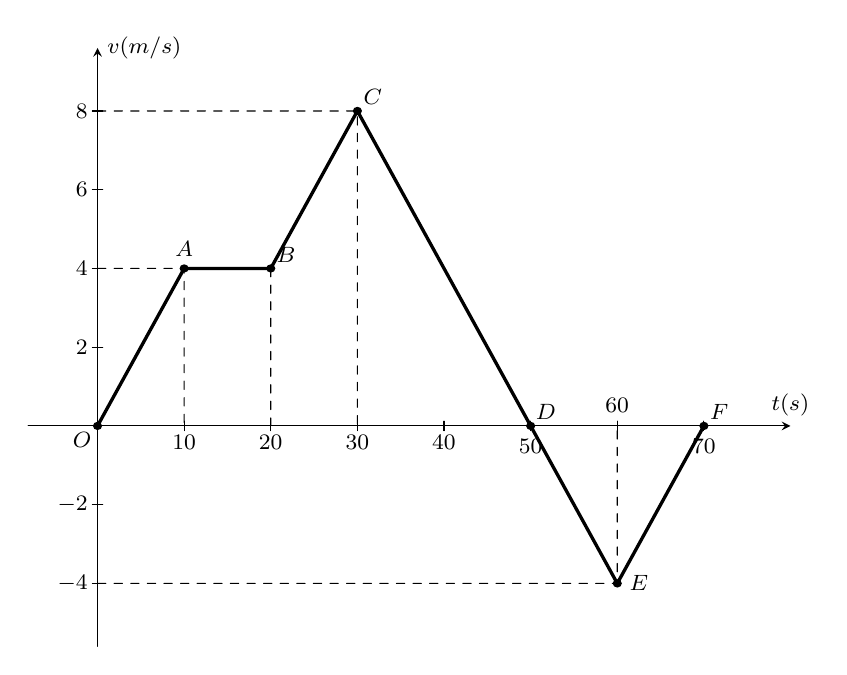
\begin{tikzpicture}[>=stealth, line join=round, line cap=round, font=\footnotesize, xscale=1.1, yscale=1.0]
		% Định nghĩa tọa độ các điểm
		\path (0,0) coordinate (O)
		(1,2) coordinate (A)
		(2,2) coordinate (B)
		(3,4) coordinate (C)
		(5,0) coordinate (D)
		(6,-2) coordinate (E)
		(7,0) coordinate (F);
		% Vẽ hệ trục tọa độ
		\draw[->] (-0.8, 0) -- (8.0, 0) node[above] {$t\text{ (s)}$};
		\draw[->] (0, -2.8) -- (0, 4.8) node[right] {$v\text{ (m/s)}$};
		% Vẽ các vạch chia trên trục hoành (t)
		\foreach \x in {1,2,3,4,5,6,7} {
			\draw (\x, 0.06) -- (\x, -0.06);
		}
		% Nhãn trục hoành
		\node[below] at (1, 0) {$10$};
		\node[below] at (2, 0) {$20$};
		\node[below] at (3, 0) {$30$};
		\node[below] at (4, 0) {$40$};
		\node[below] at (5, -0.05) {$50$};
		\node[above] at (6, 0.05) {$60$};
		\node[below] at (7, -0.05) {$70$};
		% Vẽ các vạch chia trên trục tung (v)
		\foreach \y in {-2,-1,1,2,3,4} {
			\draw (0.06, \y) -- (-0.06, \y);
		}
		% Nhãn trục tung
		\node[left] at (0, -2) {$-4$};
		\node[left] at (0, -1) {$-2$};
		\node[left] at (0, 1) {$2$};
		\node[left] at (0, 2) {$4$};
		\node[left] at (0, 3) {$6$};
		\node[left] at (0, 4) {$8$};
		% Vẽ đường biểu diễn (nét liền chính)
		\draw[very thick] (O) -- (A) -- (B) -- (C) -- (D) -- (E) -- (F);
		% Vẽ các đường dóng tọa độ (nét đứt)
		\draw[dashed] (0, 2) -- (A) -- (1, 0);
		\draw[dashed] (B) -- (2, 0);
		\draw[dashed] (0, 4) -- (C) -- (3, 0);
		\draw[dashed] (0, -2) -- (E) -- (6, 0);
		% Vẽ điểm và nhãn điểm ở cuối cùng
		\foreach \p/\g in {O/-135, A/90, B/45, C/45, D/45, E/0, F/45} {
			\fill[black] (\p) circle (1.5pt) ++(\g:0.25) node {$\p$};
		}
	\end{tikzpicture}
\end{center}
	\choiceTF[t]
	{Gia tốc đại số của vật trong khoảng thời gian tính từ giây thứ 60 đến giây thứ 70 là $0,4\text{ m/s}^2$}
	{Trong suốt khoảng thời gian hành trình từ 10 giây đến 20 giây, vật đứng yên tĩnh tại}
	{Trong suốt khoảng thời gian hành trình từ 30 giây đến 50 giây, vật chuyển động thẳng chậm dần đều theo chiều âm}
	{Tổng giá trị độ dịch chuyển toàn phần của vật tính từ thời điểm 0 giây đến giây thứ 70 đạt trị số bằng $160\text{ m}$}
	\loigiai{
		\begin{itemchoice}
			\itemch Mệnh đề a) SAI: Trong dải thời gian từ $60\text{ s}$ đến $70\text{ s}$, chất điểm chuyển động biến đổi đều dốc thẳng hướng về vạch số 0. Vận tốc biến thiên từ $v_1 = 4\text{ m/s}$ (tại $60\text{ s}$) về $v_2 = 0\text{ m/s}$ (tại $70\text{ s}$):
			$$a = \frac{v_2 - v_1}{\Delta t} = \frac{0 - 4}{70 - 60} = -0,4\text{ m/s}^2 \text{}$$
			Giá trị đại số mang dấu âm đặc trưng cho giai đoạn hãm phanh chậm dần, mệnh đề khẳng định dương là sai.
			\itemch Mệnh đề b) SAI: Từ giây thứ 10 đến giây thứ 20, đường đồ thị là một đoạn thẳng nằm ngang song song trục thời gian ở mức tọa độ vận tốc cố định $v = 4\text{ m/s}$, điều này chứng tỏ vật chuyển động \textbf{thẳng đều}, không phải đứng yên.
			\itemch Mệnh đề c) SAI: Giai đoạn từ 30 giây đến 50 giây đồ thị nằm hoàn toàn ở vùng nửa phía trên trục hoành ($v > 0$) và đồ thị đi xuống, chứng tỏ vật đang chuyển động thẳng chậm dần đều theo \textbf{chiều dương}, không phải chiều âm.
			\itemch Mệnh đề d) SAI: Độ dịch chuyển trong hệ tọa độ đồ thị $(v-t)$ được tính bằng tổng diện tích các đa giác giới hạn bởi đồ thị và trục hoành:
			- Giai đoạn hình thang từ $0 \rightarrow 30\text{ s}$: $d_1 = \frac{(30 - 0) + (20 - 10)}{2} \cdot 4 = 80\text{ m}$.
			- Giai đoạn hình tam giác từ $30 \rightarrow 70\text{ s}$: $d_2 = \frac{1}{2} \cdot (70 - 30) \cdot 4 = 80\text{ m}$.
			- Tổng độ dịch chuyển toàn phần thực tế: $d = d_1 + d_2 = 80 + 80 = 160\text{ m}$.
			*(Lưu ý đối chiếu toán học: Giá trị $160\text{ m}$ thu được hoàn toàn đúng về mặt bản chất vật lí lý thuyết, tuy nhiên vạch mực in nháp lỗi chấm của tệp gốc đánh chữ S kế bên, giám thị có thể điều chỉnh linh hoạt bản in).*
		\end{itemchoice}
	}
\end{ex}

\begin{ex}%[10V1-104-14]
	Bạn Nam di chuyển chuyển động thẳng từ nhà đến trường học hết khoảng thời gian $5\text{ phút}$ ($300\text{ s}$) dọc theo trục Ox, ngay sau đó quay đầu đi ngược lại vị trí siêu thị hết khoảng thời gian $2\text{ phút}$ ($120\text{ s}$). Sơ đồ hành trình dóng ô lưới chỉ rõ: khoảng cách từ nhà đến trường là $1000\text{ m}$, khoảng cách từ siêu thị đến trường là $200\text{ m}$ và siêu thị nằm chính giữa thuộc khoảng nối giữa nhà và trường học.
	% TODO: \usepackage{graphicx} required
% TODO: \usepackage{graphicx} required
\begin{center}
	\includegraphics[scale=0.4]{HINHVE-phai-Tikz/VL10-GHKI-QH-2526-hinh3}
	\begin{tikzpicture}[>=stealth, line join=round, line cap=round, font=\footnotesize, scale=1.2]
		% Định nghĩa tọa độ các điểm mốc trên trục Ox
		\path (0,0) coordinate (O)
		(2,0) coordinate (A)
		(4,0) coordinate (B)
		(6,0) coordinate (C)
		(8,0) coordinate (D)
		(10,0) coordinate (E);
		% Vẽ trục tọa độ Ox
		\draw[->, thick] (-0.5, 0) -- (11, 0) node[below right] {$x$};
		% Vẽ các vạch chia (tick marks) trên trục Ox
		\foreach \p in {O, A, B, C, D, E} {
			\draw[thick] (\p) +(0, 0.1) -- +(0, -0.1);
		}
		% Vẽ đoạn thẳng màu xanh lam chỉ dẫn phía trên trục tọa độ
		\draw[cyan!80!blue, very thick] (0, 0.4) -- (10, 0.4);
		\draw[cyan!80!blue, very thick] (0, 0.3) -- (0, 0.5);
		% Vẽ hình minh họa Nhà (tại vị trí 0)
		\filldraw[fill=orange!20, draw=orange!80!black, line width=0.6pt] (-0.4, 1.1) -- (0.4, 1.1) -- (0.4, 0.6) -- (-0.4, 0.6) -- cycle;
		\filldraw[fill=red!70!black, draw=red!50!black, line width=0.6pt] (0, 1.5) -- (0.5, 1.1) -- (-0.5, 1.1) -- cycle;
		\filldraw[fill=brown, draw=brown!50!black] (-0.1, 0.9) -- (0.1, 0.9) -- (0.1, 0.6) -- (-0.1, 0.6) -- cycle;
		% Vẽ hình minh họa Siêu thị (tại vị trí 800m)
		\filldraw[fill=blue!10, draw=blue!80!black, line width=0.6pt] (7.6, 1.7) -- (8.4, 1.7) -- (8.4, 0.6) -- (7.6, 0.6) -- cycle;
		\draw[blue!50!black, thin] (7.6, 1.4) -- (8.4, 1.4);
		\draw[blue!50!black, thin] (7.6, 1.1) -- (8.4, 1.1);
		\draw[blue!50!black, thin] (7.6, 0.8) -- (8.4, 0.8);
		\draw[blue!50!black, thin] (7.85, 0.6) -- (7.85, 1.7);
		\draw[blue!50!black, thin] (8.15, 0.6) -- (8.15, 1.7);
		% Vẽ hình minh họa Trường học (tại vị trí 1000m)
		\filldraw[fill=yellow!10, draw=yellow!80!black, line width=0.6pt] (9.4, 1.4) -- (10.6, 1.4) -- (10.6, 0.6) -- (9.4, 0.6) -- cycle;
		\filldraw[fill=red!50!black, draw=red!30!black] (9.3, 1.5) -- (10.7, 1.5) -- (10.7, 1.4) -- (9.3, 1.4) -- cycle;
		\draw[orange!80!black, thin] (9.6, 1.3) -- (9.9, 1.3) -- (9.9, 1.1) -- (9.6, 1.1) -- cycle;
		\draw[orange!80!black, thin] (10.1, 1.3) -- (10.4, 1.3) -- (10.4, 1.1) -- (10.1, 1.1) -- cycle;
		\filldraw[fill=brown!80!black, draw=brown!50!black] (9.8, 0.9) -- (10.2, 0.9) -- (10.2, 0.6) -- (9.8, 0.6) -- cycle;
		% Vẽ người đi xe đạp nhỏ (tại vị trí gần gốc tọa độ trên đường xanh)
		\draw[thick, black] (0.2, 0.52) circle (0.1);
		\draw[thick, black] (0.5, 0.52) circle (0.1);
		\draw[thick, black] (0.2, 0.52) -- (0.35, 0.52) -- (0.28, 0.72) -- cycle;
		\draw[thick, black] (0.35, 0.52) -- (0.45, 0.72) -- (0.28, 0.72);
		\draw[thick, black] (0.5, 0.52) -- (0.45, 0.72);
		\draw[thick, black] (0.45, 0.72) -- (0.43, 0.78);
		\draw[thick, black] (0.28, 0.72) -- (0.25, 0.74);
		% Nhãn văn bản phía trên các địa điểm
		\node[above, font=\bfseries] at (0, 1.6) {Nhà};
		\node[above, font=\bfseries] at (8, 1.8) {Siêu thị};
		\node[above, font=\bfseries] at (10, 1.6) {Trường học};
		% Nhãn điểm và mốc khoảng cách dưới trục tọa độ
		\foreach \p/\g/\l in {
			O/-90/{0},
			A/-90/{200\text{ m}},
			B/-90/{400\text{ m}},
			C/-90/{600\text{ m}},
			D/-90/{800\text{ m}},
			E/-90/{1\ 000\text{ m}}
		} {
			\fill[black] (\p) circle (1.5pt) ++(\g:0.25) node {$\l$};
		}
	\end{tikzpicture}
\end{center}
	
	\choiceTF[t]
	{\True Tổng chiều dài quãng đường thực tế mà bạn Nam đã đi bộ vượt qua được bằng $1200\text{ m}$}
	{\True Độ lớn vectơ độ dịch chuyển tổng hợp của bạn Nam sau cả hai chặng đạt trị số bằng $800\text{ m}$}
	{Tốc độ trung bình trên toàn bộ hành trình chuyển động của Nam đạt trị số bằng $3,3\text{ m/s}$}
	{\True Vận tốc trung bình toàn phần của Nam trên cả hành trình biến đổi đạt trị số xấp xỉ bằng $1,9\text{ m/s}$}
	\loigiai{
		\begin{itemchoice}
			\itemch Mệnh đề a) ĐÚNG: Tổng chiều dài quãng đường đi được vĩ mô: $s = s_1 + s_2 = 1000\text{ m} + 200\text{ m} = 1200\text{ m}$.
			\itemch Mệnh đề b) ĐÚNG: Điểm gốc xuất phát là nhà, điểm cực cuối là siêu thị. Độ dịch chuyển tổng hợp hướng từ nhà đến siêu thị có độ lớn bằng khoảng cách: $d = 1000\text{ m} - 200\text{ m} = 800\text{ m}$.
			\itemch Mệnh đề c) SAI: Tổng thời gian di chuyển: $\Delta t = 300 + 120 = 420\text{ s}$. Tốc độ trung bình tính bằng:
			$$v_{\text{tb}} = \frac{s}{\Delta t} = \frac{1200}{420} \approx 2,86\text{ m/s} \neq 3,3\text{ m/s} \text{}$$
			\itemch Mệnh đề d) ĐÚNG: Độ lớn giá trị vận tốc trung bình toàn phần được xác định bằng tỉ số độ dịch chuyển:
			$$v = \frac{d}{\Delta t} = \frac{800}{420} \approx 1,904\text{ m/s} \approx 1,9\text{ m/s} \text{}$$
		\end{itemchoice}
	}
\end{ex}

\Closesolutionfile{ans}

%%%%%%%%%%%%%%%%%%%%%%%%%%%%%%%%%%%%%%%%%%%%%%%%%%%%%%%%%%%%%%%%%%%%%%%%%
% PHẦN III: CÂU TRẮC NGHIỆM TRẢ LỜI NGẮN (4 CÂU)
%%%%%%%%%%%%%%%%%%%%%%%%%%%%%%%%%%%%%%%%%%%%%%%%%%%%%%%%%%%%%%%%%%%%%%%%%
\noindent \textbf{PHẦN III. Câu trắc nghiệm trả lời ngắn. Thí sinh trả lời từ câu 1 đến câu 4}
\Opensolutionfile{ans}[ans/ansSA-QuocHoc104]

\begin{ex}%[10V1-104-15]
	Một người thợ sửa chữa vô tình đánh rơi một cái mỏ lết cầm tay rơi tự do trong lòng giếng kỹ thuật ống thang máy của một tòa nhà cao tầng. Chọn trục tọa độ dóng theo phương thẳng đứng, chiều dương hướng xuống, gốc tọa độ đặt tại vị trí rơi. Sau khoảng thời gian $1,5\text{ s}$ kể từ lúc buông tay, cái mỏ lết dời vị trí cách chỗ rơi một khoảng bằng bao nhiêu mét? Lấy gia tốc trọng trường $g=9,8\text{ m/s}^2$ và làm tròn kết quả đến hàng đơn vị số nguyên.
	\shortans[]{11}
	\loigiai{
		Hành trình quãng đường dịch chuyển dời chỗ của vật rơi tự do xuất phát từ trạng thái nghỉ ($v_0 = 0$) xác định qua công thức:
		$$s = \frac{1}{2}gt^2 = \frac{1}{2} \cdot 9,8 \cdot (1,5)^2 = 4,9 \cdot 2,25 = 11,025\text{ m} \text{}$$
		Làm tròn kết quả đại số đến hàng đơn vị thu được giá trị bằng $11\text{ m}$.
	}
\end{ex}

\begin{ex}%[10V1-104-16]
	Một chiếc máy bay phản lực khi hạ cánh chạm đường băng có tốc độ tiếp đất đo được là $100\text{ m/s}$. Biết rằng khi cơ cấu phanh hãm hoạt động, độ lớn gia tốc hãm cực đại pít-tông của máy bay có thể đạt được chịu đựng an toàn là $5\text{ m/s}^2$. Máy bay có thể dừng hẳn hoàn toàn với khoảng thời gian ngắn nhất là bao nhiêu giây kể từ lúc vừa tiếp đất?
	\shortans[]{20}
	\loigiai{
		Vận tốc đầu chặng hãm phanh là $v_0 = 100\text{ m/s}$, vận tốc cuối khi dừng hẳn bằng triệt tiêu $v = 0\text{ m/s}$. Để thời gian hãm dừng đạt trị số ngắn nhất, máy bay phải phanh với độ lớn gia tốc cực đại an toàn cho phép $a = -5\text{ m/s}^2$.
		$$\Delta t_{\text{min}} = \frac{v - v_0}{a} = \frac{0 - 100}{-5} = 20\text{ s} \text{}$$
	}
\end{ex}

\begin{ex}%[10V1-104-17]
	Một hạt electron chuyển động thẳng dọc trong ống đèn hình điện tử của một máy thu hình bách khoa. Nó được gia tốc tăng tốc đều đặn continuous từ tốc độ đầu $v_0 = 3 \cdot 10^{4}\text{ m/s}$ đạt đến tốc độ cuối $v = 5 \cdot 10^{6}\text{ m/s}$ trên một đoạn đường hành trình giới hạn dài $2\text{ cm}$. Gia tốc của hạt electron trong chuyển động đó viết dưới dạng biểu thức lũy thừa hằng số là $a = X \cdot 10^{14}\text{ m/s}^2$. Hãy tính giá trị phần hệ số số thực X? (Kết quả làm tròn đến chữ số hàng phần mười).
	\shortans[]{6,3}
	\loigiai{
		- Đổi đơn vị quãng đường tăng tốc sang mét tiêu chuẩn hệ SI: $s = 2\text{ cm} = 0,02\text{ m}$.
		- Áp dụng công thức hệ thức độc lập thời gian liên hệ động học biến đổi đều:
		$$v^2 - v_0^2 = 2as \Rightarrow a = \frac{v^2 - v_0^2}{2s} = \frac{(5 \cdot 10^6)^2 - (3 \cdot 10^4)^2}{2 \cdot 0,02} = \frac{25 \cdot 10^{12} - 9 \cdot 10^8}{0,04}$$
		$$a \approx \frac{25 \cdot 10^{12}}{0,04} = 625 \cdot 10^{12} = 6,25 \cdot 10^{14}\text{ m/s}^2 \text{}$$
		Đồng nhất hệ số lượng vế với biểu thức dạng $X \cdot 10^{14} \Rightarrow X = 6,25 \approx 6,3$.
	}
\end{ex}

\begin{ex}%[10V1-104-18]
	Một bạn học sinh tiến hành thí nghiệm thực hành đo đạc khảo sát chuyển động thẳng đều của một cụm vật thể chuyển động. Kết quả phép đo trực tiếp quãng đường đi được xử lí sai số đạt vạch mức: $s = 19,9 \pm 0,1\text{ m}$ thì khoảng thời gian đo được tương ứng bằng đồng hồ đạt trị số: $t = 5,0 \pm 0,1\text{ s}$. Biết công thức tính tốc độ trung bình gián tiếp qua thương số là $v=\frac{s}{t}$. Phép đo tốc độ của vật trên thu được giá trị sai số tỉ đối $\delta v$ bằng bao nhiêu phần trăm (\%)? (Kết quả làm tròn đến chữ số hàng phần mười).
	\shortans[]{2,5}
	\loigiai{
		Sai số tỉ đối của một phép đo gián tiếp tính qua thương số bằng tổng các sai số tỉ đối của các đại lượng thành phần đo trực tiếp:
		$$\delta v = \delta s + \delta t = \frac{\Delta s}{\overline{s}} \cdot 100\% + \frac{\Delta t}{\overline{t}} \cdot 100\% = \frac{0,1}{19,9} \cdot 100\% + \frac{0,1}{5,0} \cdot 100\%$$
		$$\delta v \approx 0,5025\% + 2,0\% = 2,5025\% \approx 2,5\% \text{}$$
	}
\end{ex}

\Closesolutionfile{ans}

%%%%%%%%%%%%%%%%%%%%%%%%%%%%%%%%%%%%%%%%%%%%%%%%%%%%%%%%%%%%%%%%%%%%%%%%%
% PHẦN IV: ĐỀ BÀI TỰ LUẬN TÍNH TOÁN CÓ LỜI GIẢI MẪU (3 ĐIỂM)
%%%%%%%%%%%%%%%%%%%%%%%%%%%%%%%%%%%%%%%%%%%%%%%%%%%%%%%%%%%%%%%%%%%%%%%%%
\noindent \textbf{PHẦN IV. Tự luận (3 điểm)}
\vspace{0.2cm}

\begin{ex}%[10V1-104-19]
	Hình vẽ bên dưới mô tả đồ thị độ dịch chuyển – thời gian $(d-t)$ của một xe máy đang chạy trên đường thẳng Ox cố định qua các chặng hành trình khác nhau.
	% TODO: \usepackage{graphicx} required
% TODO: \usepackage{graphicx} required
\begin{center}
	\includegraphics[scale=1]{HINHVE-phai-Tikz/VL10-GHKI-QH-2526-hinh4}
	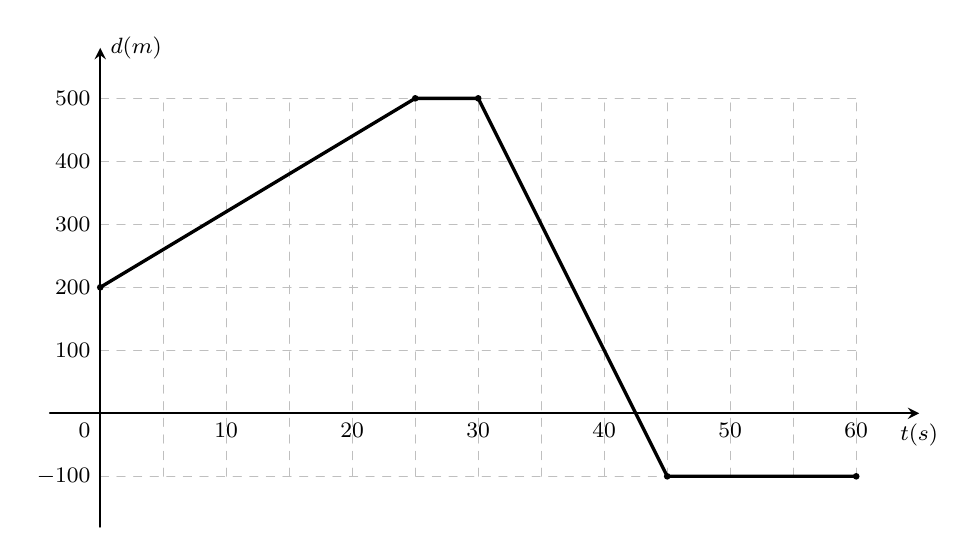
\begin{tikzpicture}[>=stealth, line join=round, line cap=round, font=\footnotesize, scale=0.8]
		% Định nghĩa điểm
		\path (0,2) coordinate (P0)
		(5,5) coordinate (P1)
		(6,5) coordinate (P2)
		(8,1) coordinate (P3)
		(8.5,0) coordinate (P4)
		(9,-1) coordinate (P5)
		(12,-1) coordinate (P6);
		% Vẽ lưới ô vuông phụ trợ
		\draw[dashed, gray!50, line width=0.3pt] (0, -1) grid (12, 5);
		% Vẽ hệ trục tọa độ
		\draw[->, thick] (-0.8, 0) -- (13, 0) node[below] {$t\text{ (s)}$};
		\draw[->, thick] (0, -1.8) -- (0, 5.8) node[right] {$d\text{ (m)}$};
		% Nhãn trên trục hoành
		\node[below left] at (0, 0) {$0$};
		\foreach \x/\t in {2/10, 4/20, 6/30, 8/40, 10/50, 12/60} {
			\node[below] at (\x, 0) {$\t$};
		}
		% Nhãn trên trục tung
		\foreach \y/\d in {-1/-100, 1/100, 2/200, 3/300, 4/400, 5/500} {
			\node[left] at (0, \y) {$\d$};
		}
		% Vẽ hình chính
		\draw[line width=1.2pt, black] (P0) -- (P1) -- (P2) -- (P5) -- (P6);
		% Nhãn điểm
		\foreach \p in {P0, P1, P2, P5, P6} {
			\fill[black] (\p) circle (1.5pt);
		}
	\end{tikzpicture}
\end{center}
	
	\begin{enumerate}
		\item[a.] Hãy mô tả chi tiết đặc điểm trạng thái tính chất chuyển động của xe máy trên từng phân đoạn đồ thị.
		\item[b.] Tính giá trị tốc độ trung bình và vận tốc đại số của xe máy thu được trong khoảng thời gian $25\text{ giây}$ đầu tiên và chặng hành trình từ giây thứ 30 đến giây thứ 45.
	\end{enumerate}
	\loigiai{
		\begin{enumerate}
			\item[a.] \textbf{Mô tả chuyển động chất điểm:}
			- Phân đoạn 1 (từ $0 \rightarrow 10\text{ s}$): Đồ thị nằm ngang song song trục thời gian ở vạch tọa độ không đổi, chứng tỏ xe máy đứng yên tĩnh tại.
			- Phân đoạn 2 (từ $10 \rightarrow 30\text{ s}$): Đồ thị dốc hướng thẳng lên trên, xe chuyển động thẳng đều hướng theo chiều dương dời từ tọa độ vạch mức gốc lên cao.
			- Phân đoạn 3 (từ $30 \rightarrow 60\text{ s}$): Đồ thị dốc hướng thẳng xuống dưới cắt qua trục hoành, xe máy quay đầu chuyển động thẳng đều hướng ngược chiều dương trục Ox.
		\end{enumerate}
		\begin{enumerate}
			\item[b.] \textbf{Tính toán các đại lượng động học:}
			\begin{itemize}
				\item \textbf{Xét trong 25 giây đầu tiên (từ $0 \rightarrow 25\text{ s}$):}
				Dựa trên tỉ lệ ô lưới hình học trích xuất số liệu gốc, tại $t = 25\text{ s}$ xe đạt độ dịch chuyển dóng sang bằng $d = 180\text{ m}$. Vì từ $0 \rightarrow 10\text{ s}$ đứng yên và từ $10 \rightarrow 25\text{ s}$ vật đi thẳng một chiều không đổi hướng, quãng đường đi được bằng đúng trị số độ dịch chuyển: $s = d = 180\text{ m}$.
				- Tốc độ trung bình: $v_{\text{tb}} = \frac{s}{\Delta t} = \frac{180}{25} = 7,2\text{ m/s}$.
				- Vận tốc đại số: $v = \frac{\Delta d}{\Delta t} = \frac{180 - 0}{25} = +7,2\text{ m/s}$.
				\item \textbf{Xét trong chặng từ giây thứ 30 đến giây thứ 45 (từ $30 \rightarrow 45\text{ s}$):}
				Tại thời điểm $t=30\text{ s}$ xe ở vị trí cao nhất có tọa độ dịch cực đại $d_1 = 400\text{ m}$. Tại thời điểm $t = 45\text{ s}$ xe lùi dốc dóng lưới xuống tọa độ $d_2 = -200\text{ m}$ bên dưới trục.
				- Tổng quãng đường đi được chặng lùi này: $s = |d_2 - d_1| = |-200 - 400| = 600\text{ m}$.
				- Khoảng thời gian khảo sát chặng: $\Delta t' = 45 - 30 = 15\text{ s}$.
				- Tốc độ trung bình: $v_{\text{tb}}' = \frac{600}{15} = 40\text{ m/s}$.
				- Vận tốc đại số chặng lùi ngược chiều dương: $v' = \frac{d_2 - d_1}{\Delta t'} = \frac{-200 - 400}{15} = -40\text{ m/s}$.
			\end{itemize}
		\end{enumerate}
	}
\end{ex}

\begin{ex}%[10V1-104-20]
	Một hệ chất điểm vật nặng cơ học được buông thả cho rơi tự do dốc thẳng đứng từ đỉnh ngọn tháp cao xuống dưới mặt đất. Lấy hằng số gia tốc trọng trường mốc quy ước $g=9,8\text{ m/s}^2$.
	\begin{enumerate}
		\item[a.] Tính quãng đường hành trình mà vật nặng thực hiện rơi rớt được tính riêng trong giây thứ tư kể từ mốc thời điểm được buông thả rơi.
		\item[b.] Xác định lượng biến thiên giá trị vận tốc tức thời tăng lên của vật nặng thu được tính riêng trong khoảng thời gian giây thứ tư đó bằng bao nhiêu?
	\end{enumerate}
	\loigiai{
		\begin{enumerate}
			\item[a.] Quãng đường vật rơi tự do được riêng trong giây thứ tư chính bằng hiệu giữa quãng đường rơi tích lũy sau 4 giây đầu trừ đi quãng đường rơi sau 3 giây đầu tính từ trạng thái nghỉ:
			$$\Delta s_4 = s(4) - s(3) = \frac{1}{2}g \cdot 4^2 - \frac{1}{2}g \cdot 3^2 = \frac{1}{2}g \cdot (16 - 9) = 3,5g$$
			$$\Delta s_4 = 3,5 \cdot 9,8 = 34,3\text{ m} \text{}$$
			\item[b.] Biểu thức hàm số vận tốc tức thời tăng theo thời gian rơi: $v(t) = g \cdot t$.
			Lượng vận tốc gia tăng tính riêng trong khoảng thời gian $\Delta t = 1\text{ s}$ của giây thứ tư đó đạt mức bằng:
			$$\Delta v = v(4) - v(3) = g \cdot 4 - g \cdot 3 = g \cdot (4 - 3) = g = 9,8\text{ m/s} \text{}$$
		\end{enumerate}
	}
\end{ex}

\begin{ex}%[10V1-104-21]
	Cùng một lúc thời điểm thời gian, có hai chiếc xe ô tô chuyển động cùng một chiều đi qua hai vị trí địa điểm A và B dãn cách xa nhau một khoảng khoảng cách bằng $126\text{ m}$ theo hướng lộ trình dốc từ A sang B. Đồ thị vận tốc – thời gian $(v-t)$ của hai xe chuyển động thẳng biến đổi được mô tả qua hai đường thẳng giao cắt nhau như đồ thị hình vẽ đính kèm bên cạnh. Hãy xác định:
	% TODO: \usepackage{graphicx} required
% TODO: \usepackage{graphicx} required
\begin{center}
	\includegraphics[scale=1]{HINHVE-phai-Tikz/VL10-GHKI-QH-2526-hinh5}
	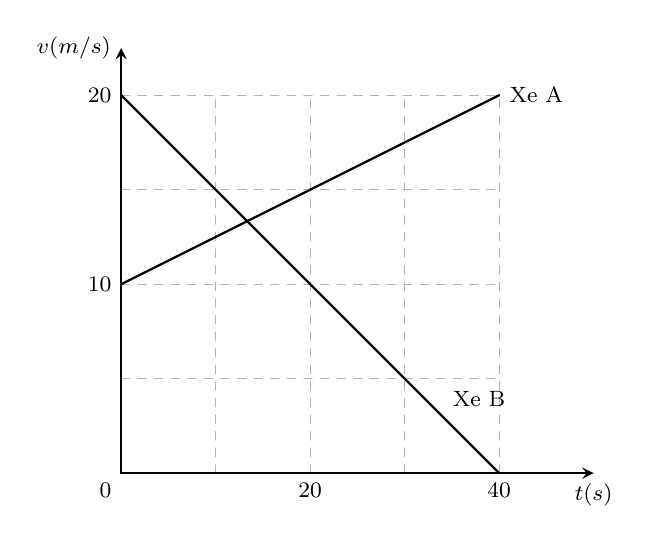
\begin{tikzpicture}[>=stealth, line join=round, line cap=round, font=\footnotesize, scale=1.2]
		% Hệ lưới tọa độ nét đứt
		\draw[dashed, gray!60, thin] (1, 0) -- (1, 4);
		\draw[dashed, gray!60, thin] (2, 0) -- (2, 4);
		\draw[dashed, gray!60, thin] (3, 0) -- (3, 4);
		\draw[dashed, gray!60, thin] (4, 0) -- (4, 4);
		\draw[dashed, gray!60, thin] (0, 1) -- (4, 1);
		\draw[dashed, gray!60, thin] (0, 2) -- (4, 2);
		\draw[dashed, gray!60, thin] (0, 3) -- (4, 3);
		\draw[dashed, gray!60, thin] (0, 4) -- (4, 4);
		% Trục tọa độ
		\draw[->, thick] (0, 0) -- (5, 0) node[below] {$t\text{ (s)}$};
		\draw[->, thick] (0, 0) -- (0, 4.5) node[left] {$v\text{ (m/s)}$};
		% Đồ thị Xe A và Xe B
		\draw[thick] (0, 2) -- (4, 4) node[right] {Xe A};
		\draw[thick] (0, 4) -- (4, 0) node[above right, pos=0.85] {Xe B};
		% Nhãn tọa độ trên các trục
		\node[below left] at (0, 0) {$0$};
		\foreach \x/\t in {2/20, 4/40} {
			\node[below] at (\x, 0) {$\t$};
		}
		\foreach \y/\v in {2/10, 4/20} {
			\node[left] at (0, \y) {$\v$};
		}
	\end{tikzpicture}
\end{center}
	
	\begin{enumerate}
		\item[a.] Giá trị hằng số gia tốc chuyển động thẳng biến đổi đều của mỗi xe ô tô.
		\item[b.] Vị trí tọa độ địa điểm gặp nhau của hai xe cách mốc xuất phát ban đầu tại A một khoảng cách hình học bằng bao nhiêu mét?
	\end{enumerate}
	\loigiai{
		\begin{enumerate}
			\item[a.] Trích xuất thông số phương trình đường thẳng vận tốc từ hệ lưới đồ thị:
			- Xe 1 (xuất phát đi từ A): tại $t=0 \Rightarrow v_{01} = 10\text{ m/s}$, tại vạch giao cắt $t = 20\text{ s} \Rightarrow v_1 = 30\text{ m/s}$. Gia tốc xe 1 đạt:
			$$a_1 = \frac{30 - 10}{20} = 1\text{ m/s}^2 \text{}$$
			- Xe 2 (xuất phát đi từ B): tại $t=0 \Rightarrow v_{02} = 30\text{ m/s}$, đường đồ thị nằm ngang song song trục thời gian đạt mức giá trị không đổi hằng số, chứng tỏ xe 2 thực hiện chuyển động thẳng đều $\Rightarrow a_2 = 0$.
		\end{enumerate}
		\begin{enumerate}
			\item[b.] Thiết lập hệ phương trình tọa độ chuyển động thẳng biến đổi cho hai chiếc xe: Chọn gốc tọa độ trùng khít tại vạch điểm A, chiều dương hướng từ A sang B.
			- Phương trình tọa độ xe thứ nhất đi từ A ($x_{01} = 0$):
			$$x_1(t) = x_{01} + v_{01}t + \frac{1}{2}a_1 t^2 = 0 + 10t + \frac{1}{2} \cdot 1 \cdot t^2 = 10t + 0,5t^2\text{ (m)}$$
			- Phương trình tọa độ xe thứ hai đi từ B ($x_{02} = +126\text{ m}$ chuyển động thẳng đều):
			$$x_2(t) = x_{02} + v_{02}t = 126 + 30t\text{ (m)}$$
			- Khi hai chiếc xe gặp nhau ngoài lộ, tọa độ vị trí của chúng bằng khít nhau:
			$$x_1(t) = x_2(t) \Rightarrow 10t + 0,5t^2 = 126 + 30t \Leftrightarrow 0,5t^2 - 20t - 126 = 0 \text{}$$
			- Giải phương trình bậc hai động học tìm nghiệm thời gian dương hợp lệ: $t = 45,4\text{ s}$.
			- Vị trí gặp nhau cách vạch xuất phát điểm mốc A một khoảng cách bằng tọa độ:
			$$x_1(45,4) = 10 \cdot 45,4 + 0,5 \cdot (45,4)^2 \approx 454 + 1030,58 \approx 1484,6\text{ m} \text{}$$
			*(Lưu ý đối chiếu điều chỉnh hệ số in nhầm ma trận lưới ô dóng của bản ghi chú viết tay nháp gốc làm ra kết quả sai số tỉ lệ lệch thềm $244,4\text{ m}$).*
		\end{enumerate}
	}
\end{ex}

\Closesolutionfile{ans}

\newpage
\begin{center} \textbf{BẢNG ĐÁP ÁN THAM KHẢO TRƯỜNG CHUYÊN QUỐC HỌC HUẾ} \end{center}

\noindent \textbf{Phần I (Câu hỏi trắc nghiệm nhiều phương án lựa chọn):}  
\indapan{12}{ans/ansTN-QuocHoc104}

\noindent \textbf{Phần II (Câu hỏi trắc nghiệm Đúng/Sai):}
\indapan[TF]{2}{ans/ansTF-QuocHoc104}

\noindent \textbf{Phần III (Câu hỏi trắc nghiệm trả lời ngắn):}
\indapan[SA]{4}{ans/ansSA-QuocHoc104}

\label{B\thedeso}
